\chapter{Results}
\begin{toReview}
Mostrare i risultati delle varie fasi e infine le analisi utili per l'attribuzione
    \section{pre processing}
    Mostrare i risultati del pre processing.
    \begin{itemize}
        \item serie di fourier applicate a griglie sintetiche per dedurre quali sono le frequenze di nostro interesse: griglie dritte e ruotate, griglie chiare e scure, griglie con elementi inquinanti, confronto tra teoria e aspettativa
        \item serie di fourier applicate a immagini vere, confronto con le immagini sintetiche
        \item risultati della pulizia dei quadretti
    \end{itemize}
    \section{synthesis}
    Mostrare una piccola analisi delle sintesi ottenute e della velocità del programma
    \section{analysis}
    Mostrare i risultati delle analisi con i vari clustering
\end{toReview}



\begin{figure}
	\centering
	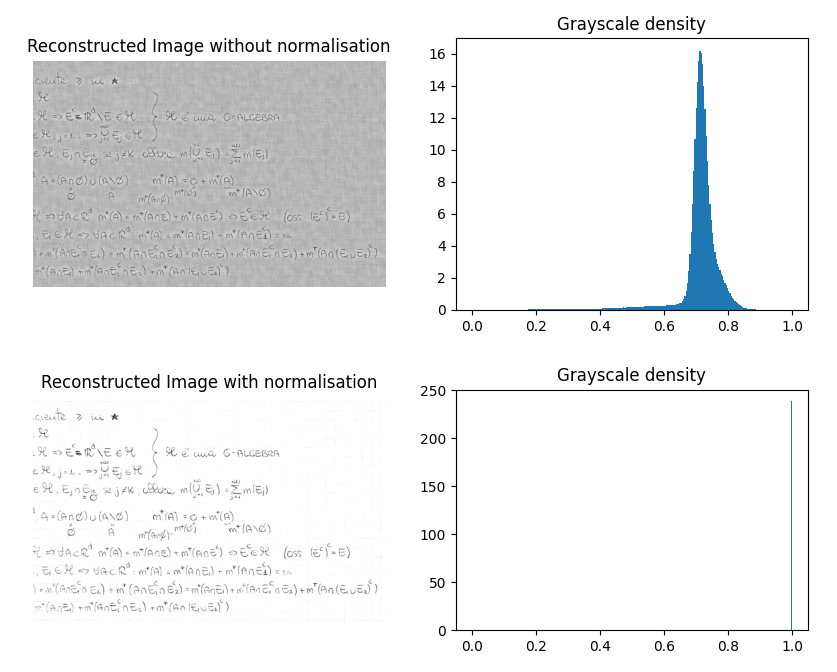
\includegraphics[width=\linewidth]{Figures/first_reconstruct.png}
	\caption{Come si osserva i grigi si sono molto avvicinati tra loro dopo \gls{fft}, ma è possibile ribilanciare i colori confrontandoli con l'immagine originale.}
	\label{fig:first_reconstruct}
\end{figure}
